\documentclass[10 pt]{beamer}
\usetheme{Madrid}
\usepackage[utf8]{inputenc}
\usepackage{xspace}
\usepackage{graphicx,graphics} 
\usepackage{color}
\usepackage{amsmath}
\usepackage{amsfonts}
\usepackage{amssymb}
\usepackage{amsthm}
\usepackage{tabularx}
\usepackage{algorithm}
\usepackage{algorithmic}
\usepackage{longtable}
\usepackage{complexity}
\usepackage{tkz-graph}
\usepackage{float}
\usepackage{multicol}
\usepackage{setspace}
\usepackage[absolute,overlay]{textpos}
\graphicspath{{fig/}}

\tikzset{
  LabelStyle/.style = { rectangle, rounded corners, draw,
                       font = \bfseries },
  EdgeStyle/.append style = {-} }
\title{ Deterministic architectures for low latency in 5G and beyond systems}

\author{{\bf Maël~Guiraud}}


\institute[Nokia Bell Labs, DAVID-UVSQ] 
{
  Nokia Bell Labs France - DAVID, Universit\'e de Versailles Saint Quentin
   \\
}

\subject{Theoretical Computer Science}

\begin{document}


\begin{frame}

  \titlepage
  \centering
  
\includegraphics [width=25mm]{logon.png} \hspace{1cm} 
\includegraphics [width=17.5mm]{logod.png} \\
\end{frame}




\begin{section}{Introduction}

\begin{frame}{Context}


  \centering
  
  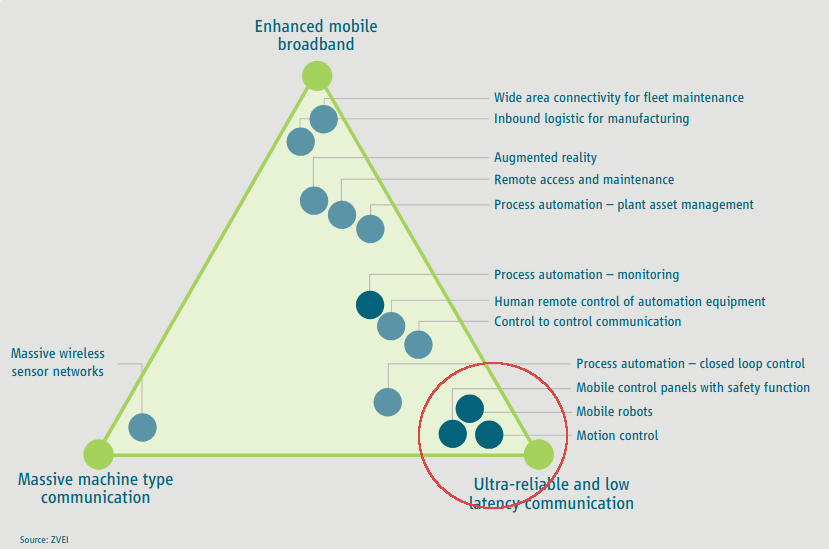
\includegraphics[scale=0.4]{usecases.png}
  

\end{frame}





\begin{frame}{Use case: Cloud-RAN}
  \centering
  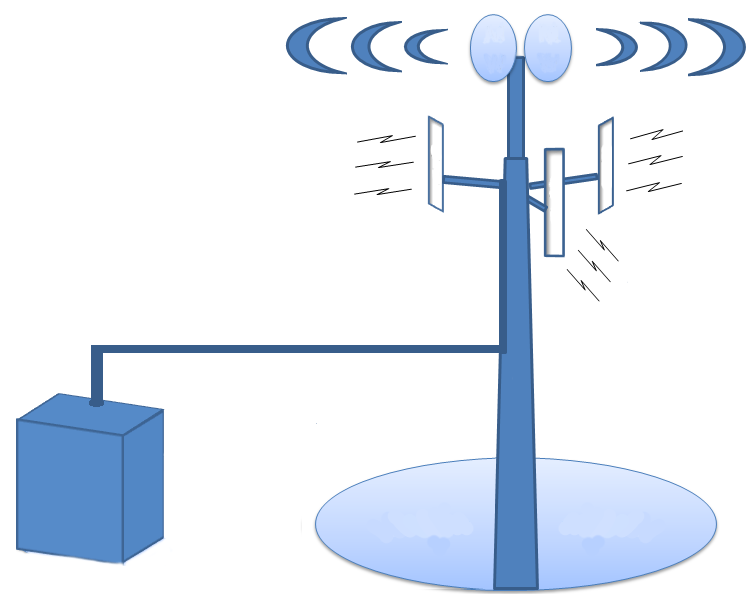
\includegraphics[scale=0.2]{cloudbts.png}\\
  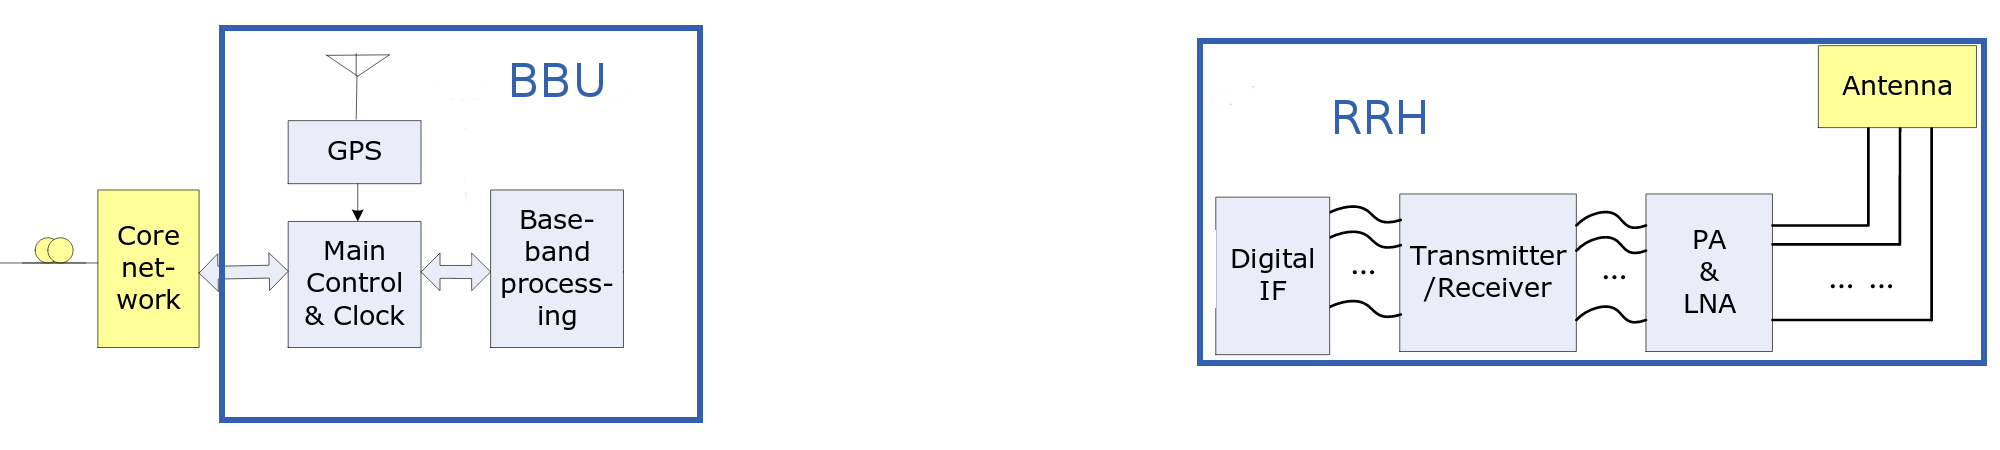
\includegraphics[scale=0.175]{BBURRH.png}
  
   RU=RRH, Distributed/Centralized Unit=BBU
\end{frame}



\begin{frame}{Use case: Cloud-RAN}
  \centering
  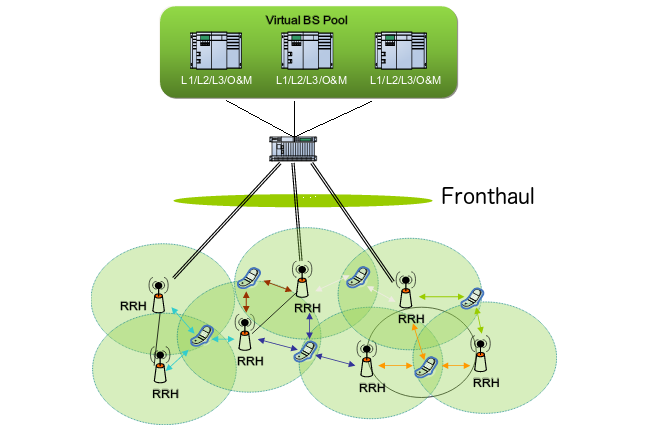
\includegraphics[scale=0.3]{CRAN}\\
  \vspace{0.5cm}
  \pause
  C-RAN aims to mutualize the computation ressources.
  
  \textcolor{red}{Since the processing time is constrained by protocol, the lower the transmission delay, the more important the sharing (ie. the coverage area of a data center).}
  
  \textcolor{blue}{The minimum latency allows to increase the mutualization.}
  
  
\end{frame}


\begin{frame}{Problematic}
  \centering
  
  
 \begin{multicols}{2}
Specificity of Cloud-RAN:
\vspace{1cm}
\begin{itemize}
\item \textcolor{red}{Minimize latency}: increase the cover area.
\item Periodic traffic 

\end{itemize}
\vspace{2cm}
Current approaches: \begin{itemize}
\vspace{1cm}
\item Dedicated network $\rightarrow$ Too expensive
\item Statistical multiplexing (TSN/Qbv) $\rightarrow$ \textcolor{red}{bounded latency only}
\end{itemize}
\end{multicols}

\end{frame}

\end{section}

\begin{section}{Model, Problem}

\begin{subsection}{Network Modeling}

\begin{frame}{Model}
\begin{center}
  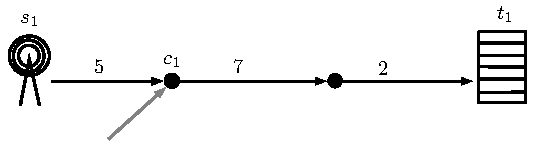
\includegraphics [width=9cm]{1routealler} 
\end{center}

\begin{itemize}
\item Network $\rightarrow$ Weighted DAG
\item  Physical Delay of a link $\rightarrow$ Weight of the arc
\item  Only the contention points are represented in the graph
\end{itemize}

\begin{center}
\scalebox{0.6}{

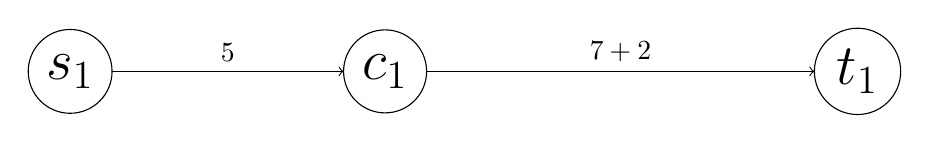
\begin{tikzpicture}
  \SetGraphUnit{5}
    \tikzset{
  EdgeStyle/.append style = {->} }
   \tikzstyle{VertexStyle}=[shape = circle, draw, minimum size = 30pt]
   \renewcommand{\VertexLightFillColor}{orange}
  \Vertex[x=0,y=0, L = {\huge $s_1$}]{s1};

\Vertex[x=10,y=0, L = {\huge $t_1$}]{t1};

  \Vertex[x=4,y=0, L = {\huge $c_1$}]{c1}
  
 %\SetVertexNoLabel
  %\Vertex[x=4,y=2]{n1}

 % \Edge[label = $5$](s1)(c1)
 % \Edge[label = $7 + 2$](c1)(t1)
  \path (s1) edge [->] node[anchor=south]{$5$} (c1);
\path (c1) edge [->] node[anchor=south]{$7+2$} (t1);

 


\end{tikzpicture}
}
  \end{center}


 \end{frame}
 
\begin{frame}{Model}
Both ways: from RRH to BBU (forward) then from BBU to RRH (backward)
 \begin{center}
  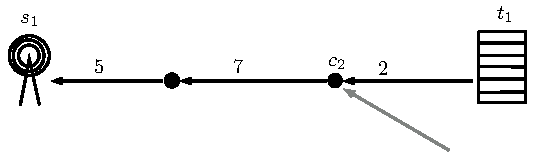
\includegraphics [width=9cm]{1routeretour} 
\end{center}


\begin{center}
\scalebox{0.6}{

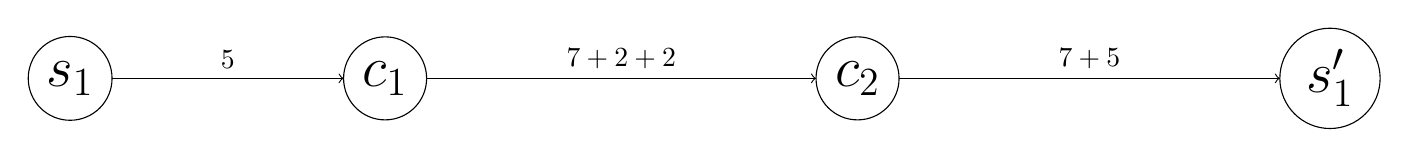
\begin{tikzpicture}
  \SetGraphUnit{5}
    \tikzset{
  EdgeStyle/.append style = {->} }
   \tikzstyle{VertexStyle}=[shape = circle, draw, minimum size = 30pt]
   \renewcommand{\VertexLightFillColor}{orange}
  \Vertex[x=0,y=0, L = {\huge $s_1$}]{s1};
\Vertex[x=16,y=0, L = {\huge $s_1'$}]{s1p};
\Vertex[x=10,y=0, L = {\huge $c_2$}]{c2};

  \Vertex[x=4,y=0, L = {\huge $c_1$}]{c1}
  
 %\SetVertexNoLabel
  %\Vertex[x=4,y=2]{n1}

  %\Edge[label = $5$](s1)(c1)
 % \Edge[label = $7 + 2+2$](c1)(c2)
 % \Edge[label = $7 + 2+2$](c1)(c2)
%\Edge[label = $7 + 5$](c2)(s1p)
 
\path (s1) edge [->] node[anchor=south]{$5$} (c1);
\path (c1) edge [->] node[anchor=south]{$7+2+2$} (c2);
\path (c2) edge [->] node[anchor=south]{$7+5$} (s1p);


\end{tikzpicture}
}
\end{center}
\end{frame}

\begin{frame}{Model}

 \begin{center}
  \includegraphics [width=7.5cm]{starfronthaul} 
\end{center}


\begin{center}
\scalebox{0.6}{

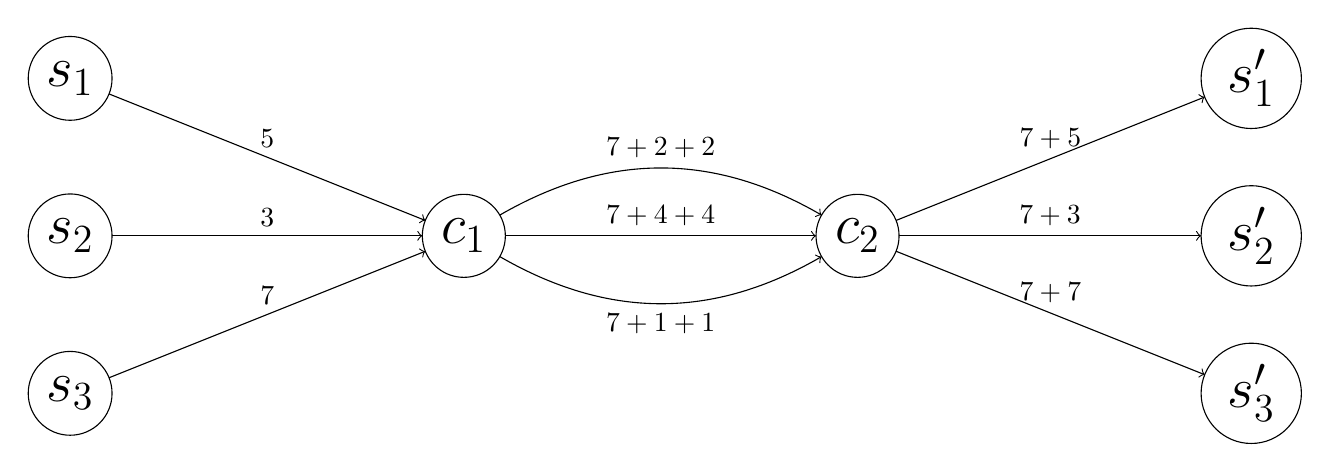
\begin{tikzpicture}
  \SetGraphUnit{5}
    \tikzset{
  EdgeStyle/.append style = {->} }
   \tikzstyle{VertexStyle}=[shape = circle, draw, minimum size = 30pt]
   \renewcommand{\VertexLightFillColor}{orange}
  \Vertex[x=0,y=4, L = {\huge $s_1$}]{s1};
  \Vertex[x=0,y=2, L = {\huge $s_2$}]{s2};
\Vertex[x=0,y=0, L = {\huge $s_3$}]{s3};
\Vertex[x=15,y=4, L = {\huge $s_1'$}]{s1p};
\Vertex[x=15,y=2, L = {\huge $s_2'$}]{s2p};
\Vertex[x=15,y=0, L = {\huge $s_3'$}]{s3p};
\Vertex[x=10,y=2, L = {\huge $c_2$}]{c2};

  \Vertex[x=5,y=2, L = {\huge $c_1$}]{c1}
  
 %\SetVertexNoLabel
  %\Vertex[x=4,y=2]{n1}

  %\Edge[label = $5$](s1)(c1)
  %\Edge[label = $7 + 4+4$](c1)(c2)
  %\Edge[label = $3$](s2)(c1)
   %\Edge[label = $7$](s3)(c1)
  %  \Edge[label = $7+3$](c2)(s2p)
 %  \Edge[label = $7+7$](c2)(s3p)
%\Edge[label = $7 + 5$](c2)(s1p)
\path (s1) edge [->] node[anchor=south]{$5$} (c1);

\path (s2) edge [->] node[anchor=south]{$3$} (c1);
\path (s3) edge [->] node[anchor=south]{$7$} (c1);
\path (c2) edge [->] node[anchor=south]{$7+3$} (s2p);
\path (c2) edge [->] node[anchor=south]{$7+7$} (s3p);

\path (c2) edge [->] node[anchor=south]{$7+5$} (s1p);

\path (c1) edge [->] node[anchor=south]{$7+4+4$} (c2);

\path (c1) edge [->,bend left=30] node[anchor=south]{$7+2+2$} (c2);
\path (c1) edge [->,bend right=30] node[anchor=north]{$7+1+1$} (c2);

  %\draw[->,line width=0.5pt] (5,2.51) parabola bend (7.5,3.5) (10,2.51);
 %\draw[->,line width=0.5pt] (5,1.49) parabola bend (7.5,0.5) (10,1.49);
 

\end{tikzpicture}
}
\end{center}
\end{frame}
 
 
 \begin{frame}{The communication process}
 
 The time is discretized.

Two fixed parameters determined by the use case.
\begin{itemize}
\item The period $P$
\item The size of a message $\tau$
\end{itemize}
\vspace{0.5cm}

Every $P$ units of time, a message of size $\tau$ is emitted from each RRH.

\vspace{0.5cm}
\begin{center}
  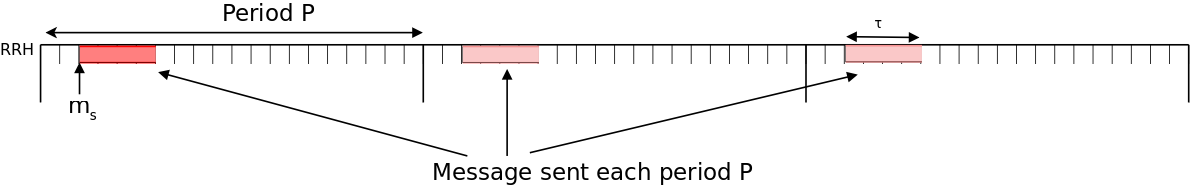
\includegraphics [width=11.5cm]{rrh} 
  \end{center}
 \vspace{0.5cm}
   
   The process is \textcolor{red}{periodic} : the message is emitted in each period at the same time, called \textcolor{blue}{offset}.
   
\end{frame}


 \begin{frame}{Collisions}

\begin{center}
\scalebox{0.6}{

\begin{tikzpicture}
  \SetGraphUnit{5}
    \tikzset{
  EdgeStyle/.append style = {->} }
   \tikzstyle{VertexStyle}=[shape = circle, draw, minimum size = 30pt]
   \renewcommand{\VertexLightFillColor}{orange}
  \Vertex[x=0,y=3, L = {\huge $s_2$}]{a3};

  \Vertex[x=0,y=6, L = {\huge $s_1$}]{a1}


  \Vertex[x=4,y=3, L = {\huge $c$}]{c}
   
 \SetVertexNoLabel
\Vertex[x=7,y=3]{d}

      \Edge(c)(d)
  \tikzset{
  EdgeStyle/.append style = {blue} }
  \Edge[label = 5](a1)(c)   
 
  
    \tikzset{
  EdgeStyle/.append style = {red} }
    \Edge[label = 3](a3)(c)
  
      
       \node (0) at (5,2){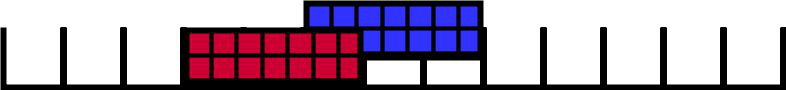
\includegraphics[scale=0.2]{col1.png}};


\end{tikzpicture}
}
\end{center}
\vspace{1cm}
\centering
There is a \textcolor{blue}{collision} between two routes when their messages go through the first vertex of a common arc at the same time.
\vspace{0.5cm}

 \textcolor{red}{Periodicity must be taken into consideration} 
\end{frame}

 \begin{frame}{Assignment }

 $P=13, \tau = 3$ 
 
\begin{center}
 \begin{multicols}{2}
\scalebox{0.6}{

\begin{tikzpicture}
  \SetGraphUnit{5}
    \tikzset{
  EdgeStyle/.append style = {->} }
   \tikzstyle{VertexStyle}=[shape = circle, draw, minimum size = 30pt]
   \renewcommand{\VertexLightFillColor}{orange}
  \Vertex[x=0,y=3, L = {\huge $s_2$}]{a3};

  \Vertex[x=0,y=6, L = {\huge $s_1$}]{a1}


  \Vertex[x=4,y=3, L = {\huge $c$}]{c}
  
 \SetVertexNoLabel
\Vertex[x=7,y=3]{d}

      \Edge(c)(d)

    
  \tikzset{
  EdgeStyle/.append style = {blue} }
  \Edge[label = 5](a1)(c)   
 
  
    \tikzset{
  EdgeStyle/.append style = {red} }
    \Edge[label = 3](a3)(c)
  \node (0) at (0,2.2){0};
      \node (0) at (0,5.2){0};
       \node (0) at (5,2){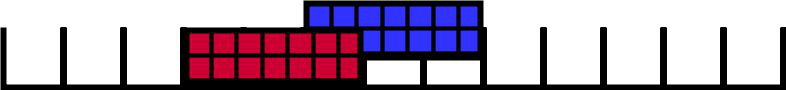
\includegraphics[scale=0.2]{col1.png}};


\end{tikzpicture}
}
\pause
\hspace{0.2cm}$\rightarrow$
\scalebox{0.6}{

\begin{tikzpicture}
  \SetGraphUnit{5}
    \tikzset{
  EdgeStyle/.append style = {->} }
   \tikzstyle{VertexStyle}=[shape = circle, draw, minimum size = 30pt]
   \renewcommand{\VertexLightFillColor}{orange}
  \Vertex[x=0,y=3, L = {\huge $s_2$}]{a3};

  \Vertex[x=0,y=6, L = {\huge $s_1$}]{a1}


  \Vertex[x=4,y=3, L = {\huge $c$}]{c}
  
 \SetVertexNoLabel
\Vertex[x=7,y=3]{d}

      \Edge(c)(d)

    
  \tikzset{
  EdgeStyle/.append style = {blue} }
  \Edge[label = 5](a1)(c)   
 
  
    \tikzset{
  EdgeStyle/.append style = {red} }
    \Edge[label = 3](a3)(c)
    \node (0) at (0,2.2){0};
      \node (0) at (0,5.2){1};
       \node (0) at (5,2){
\includegraphics[scale=0.2]{col2.png}};


\end{tikzpicture}
}
\end{multicols}
\end{center}

\vspace{1cm}
\centering
Choosing the offset such that there are no collisions.
\vspace{0.5cm}
\pause

An \textcolor{blue}{assignment} is a choice of offsets for each route without collisions.
\end{frame}
\end{subsection}



\begin{subsection}{Problem PALL}
\begin{frame}{Full process}
In each BBU, one can choose the \textcolor{blue}{waiting time} before sending back the answer.\\

\begin{center}
  \includegraphics[scale=0.7]{BBU}\\
 \end{center} 

\textbf{Problem:}

Given a routed network, a period and a message size, find an assignment such that there is no collisions.
\end {frame}
\begin{frame}
Two measures to optimize.
 \begin{multicols}{2}
PALL:
\begin{itemize}
\item The sources may send their message at different dates in the period.
\item Local latency constraint.
\item Minimizing the process time on the longest route.
\item Use cases: URLLC/Indutry 4.0
\end{itemize}
\vspace{0.5cm}
SPALL:
\begin{itemize}
\item The sources send their message at the same date: \textbf{Synchronized}.
\item Global time constraint.
\item Minimize the time between the emission of the first message and the reception of the last message.
\item use cases: C-RAN
\end{itemize}
\end{multicols}

The optimal solutions for PALL and SPALL are not the same.
\end{frame}
\end{subsection}


\end{section}

\begin{section}{Results on a common topology}

\begin{subsection}{A star routed Network}
\begin{frame}{Different topologies}

The  {\bf conflict depth} of a route is defined as the number of contention point on the route.

The conflict depth of a routed network is the maximal conflict depth of the routes in the network.
  \centering
   \begin{multicols}{2}


\includegraphics[scale=0.5]{starfronthaul}

 \vspace{1cm}
\centering
 Conflict depth $2$.
 

 

 
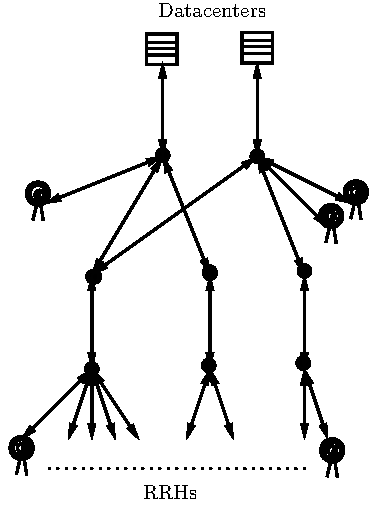
\includegraphics[scale=0.5]{extendendgraphgrey}\\
 \centering

 Conflict depth $3$ and more.

\end{multicols}
\end{frame} 

\begin{frame}{NP-Hardness}


   \begin{multicols}{2}
   PALL:
   \begin{itemize}
   \item NP-hard on conflict depth $\geq 3$: reduction from k-coloring problem
   \item NP-hard on conflict depth $2$ if the shared arc is not bidirectional.
   \end{itemize}
   
   SPALL:
   \begin{itemize}
    \item NP-hard on conflict depth $\geq 3$ 
       \item NP-hard on conflict depth $2$: reduction from two processors scheduling problem.
   \end{itemize}
   \end{multicols}

\end{frame}


\begin{frame}{Algorithmic solutions}


   \begin{multicols}{2}
   Conflict depth $2$:
   \begin{itemize}
   \item Algorithms with theoretical guarantees for moderate load.
   \item FPT algorithm based on single processor scheduling. FPT: exponential in $n$, the number of routes but linear in $P$ and $\tau$
   \end{itemize}
   \vspace{1cm}
   Conflict depth $\geq 3$:
   \begin{itemize}
    \item Local search algorithms (hill climbing, simulated anealing) 
       \item Optimized Branch and bound: computes realistic instances.
   \end{itemize}
   \end{multicols}

\end{frame}
\end{subsection}


\begin{subsection}{Results}

  
    \begin{frame}{Deterministic vs Statistic}
\centering
\vspace{-2cm}
  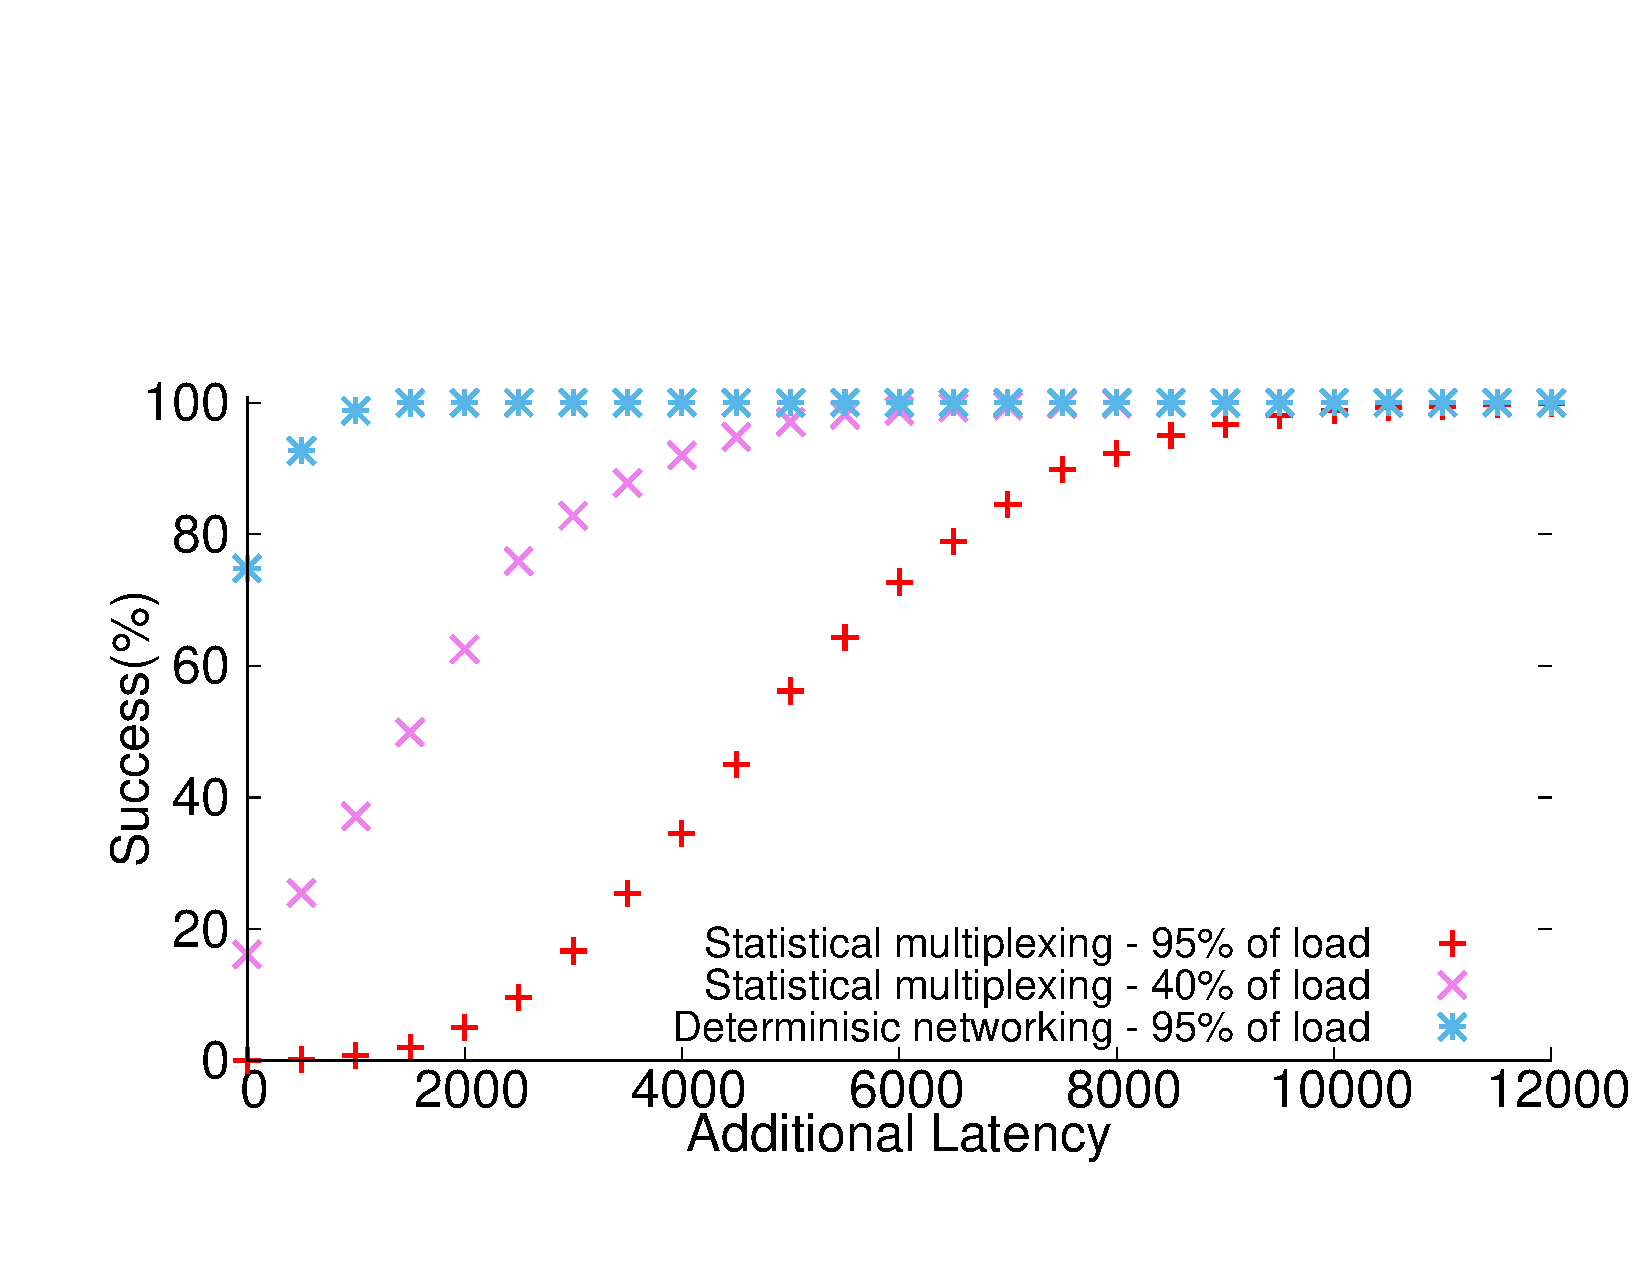
\includegraphics[scale=0.4]{stochastic.pdf}\\
  
  Conflict depth $2$ - Deterministic = optimal solution\\
  Period : $20.000$ tics 
  \end{frame}
  
      \begin{frame}{BE Latency optimization}
\centering

  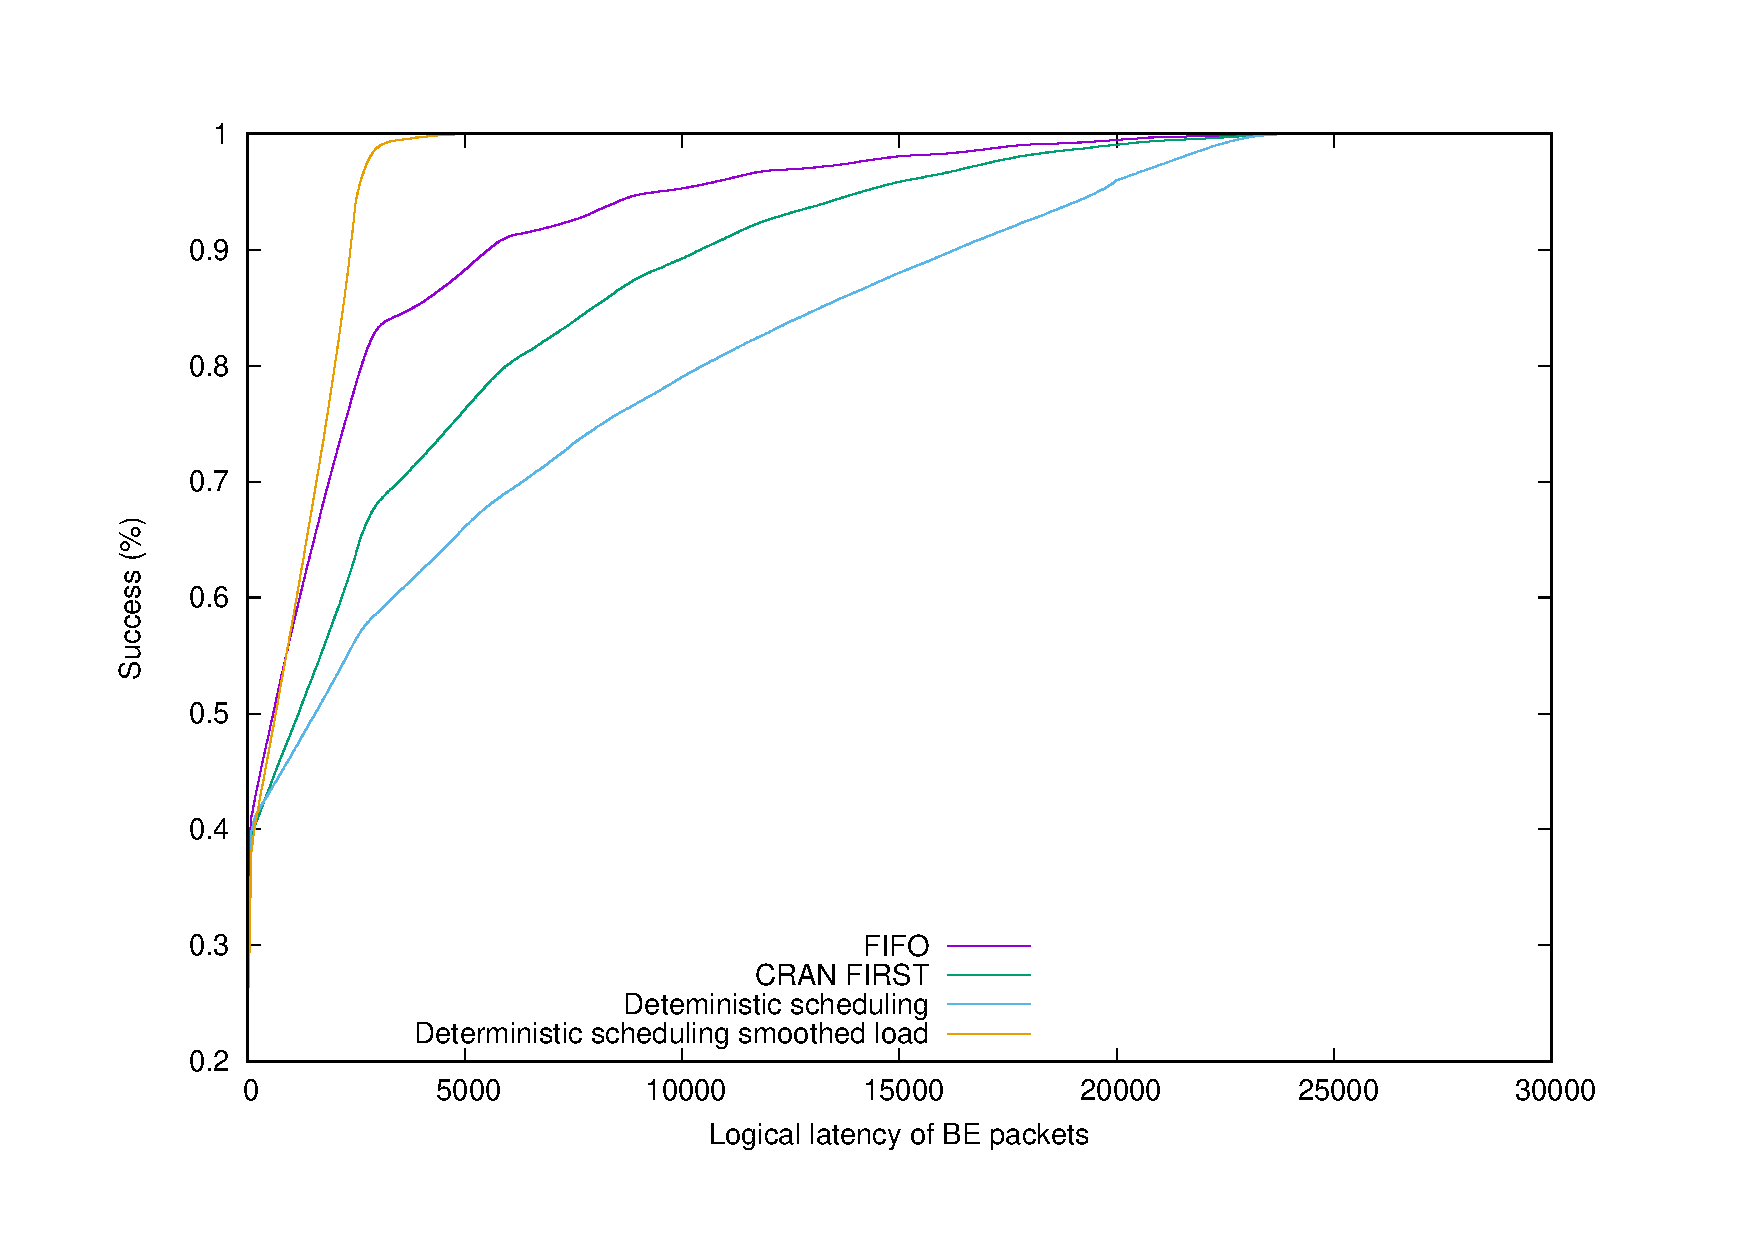
\includegraphics[scale=0.3]{res.pdf}\\
  
   Conflict depth $2$ - Deterministic = optimal solution\\
  Period : $33.000$ tics - CRAN Load : $60\%$ - BE Load $\simeq 20\%$
  \end{frame}

\end{subsection}


\end{section}


  \begin{frame}{Conclusion}
  \begin{itemize}
   \item Minimal latency allows higher area coverage: better OPEX
   \item Deterministic traffic:
     \begin{itemize}
   \item Zero contention
   \item Transparent optical transmission (i.e. without opto-electronic convertion)
   \item Energy efficiency 
  \end{itemize}
  \item Better overall traffic on loaded networks
  \end{itemize}

  \vspace{1cm}
  \pause
  Future work
\begin{itemize}
 \item Performance evaluation for conflict depth $\geq 3$
 \item Writing the PhD manuscript
\end{itemize}
 

\pause
\hspace{2cm}\huge{Thank you for your attention.}
  

\end{frame}




\end{document}
